\documentclass[
11pt, % The default document font size, options: 10pt, 11pt, 12pt
%codirector, % Uncomment to add a codirector to the title page
]{charter} 

% El títulos de la memoria, se usa en la carátula y se puede usar el cualquier lugar del documento con el comando \ttitle
\titulo{Predicción de quiebra de empresas mediante técnicas de Machine Learning} 

% Nombre del posgrado, se usa en la carátula y se puede usar el cualquier lugar del documento con el comando \degreename
%\posgrado{Carrera de Especialización en Sistemas Embebidos} 
%\posgrado{Carrera de Especialización en Internet de las Cosas} 
\posgrado{Carrera de Especialización en Inteligencia Artificial}
%\posgrado{Maestría en Sistemas Embebidos} 
%\posgrado{Maestría en Internet de las cosas}

% Tu nombre, se puede usar el cualquier lugar del documento con el comando \authorname
% IMPORTANTE: no omitir titulaciones ni tildación en los nombres, también se recomienda escribir los nombres completos (tal cual los tienen en su documento)
\autor{Ing. Gaspar Acevedo Zain}

% El nombre del director y co-director, se puede usar el cualquier lugar del documento con el comando \supname y \cosupname y \pertesupname y \pertecosupname
\director{Título y Nombre del director}
\pertenenciaDirector{pertenencia} 
\codirector{} % para que aparezca en la portada se debe descomentar la opción codirector en los parámetros de documentclass
\pertenenciaCoDirector{FIUBA}

% Nombre del cliente, quien va a aprobar los resultados del proyecto, se puede usar con el comando \clientename y \empclientename
\cliente{Nombre del cliente}
\empresaCliente{Empresa del cliente}
 
\fechaINICIO{24 de junio de 2025}		%Fecha de inicio de la cursada de GdP \fechaInicioName
\fechaFINALPlan{19 de agosto de 2025} 	%Fecha de final de cursada de GdP
\fechaFINALTrabajo{a definir}	%Fecha de defensa pública del trabajo final

\usepackage{hyperref}

\begin{document}

\maketitle
\thispagestyle{empty}
\pagebreak


\thispagestyle{empty}
{\setlength{\parskip}{0pt}
\tableofcontents{}
}
\pagebreak


\section*{Registros de cambios}
\label{sec:registro}


\begin{table}[ht]
\label{tab:registro}
\centering
\begin{tabularx}{\linewidth}{@{}|c|X|c|@{}}
\hline
\rowcolor[HTML]{C0C0C0} 
Revisión & \multicolumn{1}{c|}{\cellcolor[HTML]{C0C0C0}Detalles de los cambios realizados} & Fecha      \\ \hline
0      & Creación del documento                                 &\fechaInicioName \\ \hline
1      & Se completa hasta el punto 5 inclusive                & {6} de {Julio} de 2025 \\ \hline
2      & Se completa hasta el punto 9 inclusive                & {14} de {Julio} de 2025 \\ \hline
%		  Se puede agregar algo más \newline
%		  En distintas líneas \newline
%		  Así                                                    & {día} de {mes} de 202X \\ \hline
%3      & Se completa hasta el punto 12 inclusive                & {día} de {mes} de 202X \\ \hline
%4      & Se completa el plan	                                 & {día} de {mes} de 202X \\ \hline

% Si hay más correcciones pasada la versión 4 también se deben especificar acá

\end{tabularx}
\end{table}

\pagebreak



\section*{Acta de constitución del proyecto}
\label{sec:acta}

\begin{flushright}
Buenos Aires, \fechaInicioName
\end{flushright}

\vspace{2cm}

Por medio de la presente se acuerda con el \authorname\hspace{1px} que su Trabajo Final de la \degreename\hspace{1px} se titulará ``\ttitle'' y consistirá en {el desarrollo de una herramienta basada en Machine Learning que permita predecir si una empresa puede entrar en quiebra o no}. El trabajo tendrá un presupuesto preliminar estimado de {604} horas y un costo estimado de \textcolor{red}{\$ XXX}, con fecha de inicio el \fechaInicioName\hspace{1px} y fecha de presentación pública el \fechaFinalName.

Se adjunta a esta acta la planificación inicial.

\vfill

% Esta parte se construye sola con la información que hayan cargado en el preámbulo del documento y no debe modificarla
\begin{table}[ht]
\centering
\begin{tabular}{ccc}
\begin{tabular}[c]{@{}c@{}}Dr. Ing. Ariel Lutenberg \\ Director posgrado FIUBA\end{tabular} & \hspace{2cm} & \begin{tabular}[c]{@{}c@{}}\clientename \\ \empclientename \end{tabular} \vspace{2.5cm} \\ 
\multicolumn{3}{c}{\begin{tabular}[c]{@{}c@{}} \supname \\ Director del Trabajo Final\end{tabular}} \vspace{2.5cm} \\
\end{tabular}
\end{table}


\section{1. Descripción técnica-conceptual del proyecto a realizar}
\label{sec:descripcion}

%\begin{consigna}{red} % ELIMINAR \begin{consigna}{red} y \end{consigna}{red} en las secciones que vayan completando para cada entrega parcial.
Este proyecto consiste en un emprendimiento personal cuyo objetivo es utilizar técnicas de aprendizaje de máquina para detectar si una empresa puede entrar en quiebra o no. Este análisis puede resultar de gran interés y utilidad para distintos participantes del mercado financiero. Por ello, se considerarán como potenciales usuarios finales a empresas especializadas en finanzas, en inversiones, en prestación de seguros, entre otras.

Para llevar a cabo al mismo, se utilizará un \textit{dataset} publicado por el \href{https://www.tejwin.com/en/}{Taiwan Economic Journal}, el cual contiene información financiera de empresas del mercado de Taiwán entre los años 1999 y 2009. Al ser estos datos públicos, hoy en día existen soluciones que exploran esta temática. Algunas de ellas hacen uso de modelos de \textit{machine learning} tales como \textit{SVM} y \textit{XGBoost}, junto con algunas técnicas de preprocesamiento de datos como \textit{Smote} y de búsqueda de hiperparámetros como \textit{Random Search}.

Con el fin de diferenciarse de estas soluciones, se propone implementar el marco de trabajo basado en \textit{MLFlow} definido en la figura \ref{fig:diagBloques}. En el mismo se detallan una serie de etapas cuyas salidas se refinarán durante distintas iteraciones. Esto permitirá explorar diversas técnicas de preprocesamiento de datos, búsqueda de hiperparámetros y modelos de \textit{machine learning} que ayuden a lograr el objetivo de este proyecto.

El proyecto se encuentra en la etapa de planificación. El desarrollo e implementación del mismo se realizará en distintas etapas. Se comenzará con un análisis exploratorio de datos, que nos permitirá conocer mejor al dataset en cuestión. Luego, se realizarán diversas iteraciones sobre las siguientes etapas:

\begin{itemize}
	\item Preprocesamiento de datos: en la primer iteración se implementarán técnicas de tratamiento de nulos y desbalance de clases. En las siguientes iteraciones, se estudiarán técnicas de extracción e ingeniería de features.
	\item Entrenamiento de modelos: se implementará un modelo distinto en cada iteración. Los modelos a explorar son regresión logística, \textit{SVM} y \textit{XGBoost}. También se explorará la optimización de hiperparámetros mediante búsqueda bayesiana.
	\item Evaluación y refinamiento: en esta etapa se evaluará al modelo entrenado en la etapa anterior. Se generarán métricas que permitirán compararlo con resultados obtenidos en otras iteraciones.
\end{itemize}

La innovación de este proyecto radica en el uso del marco de trabajo definido en la figura \ref{fig:diagBloques}. Éste proporciona un ambiente productivo, reproducible y escalable, en donde se podrán analizar diversas técnicas de aprendizaje de máquina para detectar si una empresa puede entrar en quiebra o no.

\begin{figure}[htpb]
\centering 
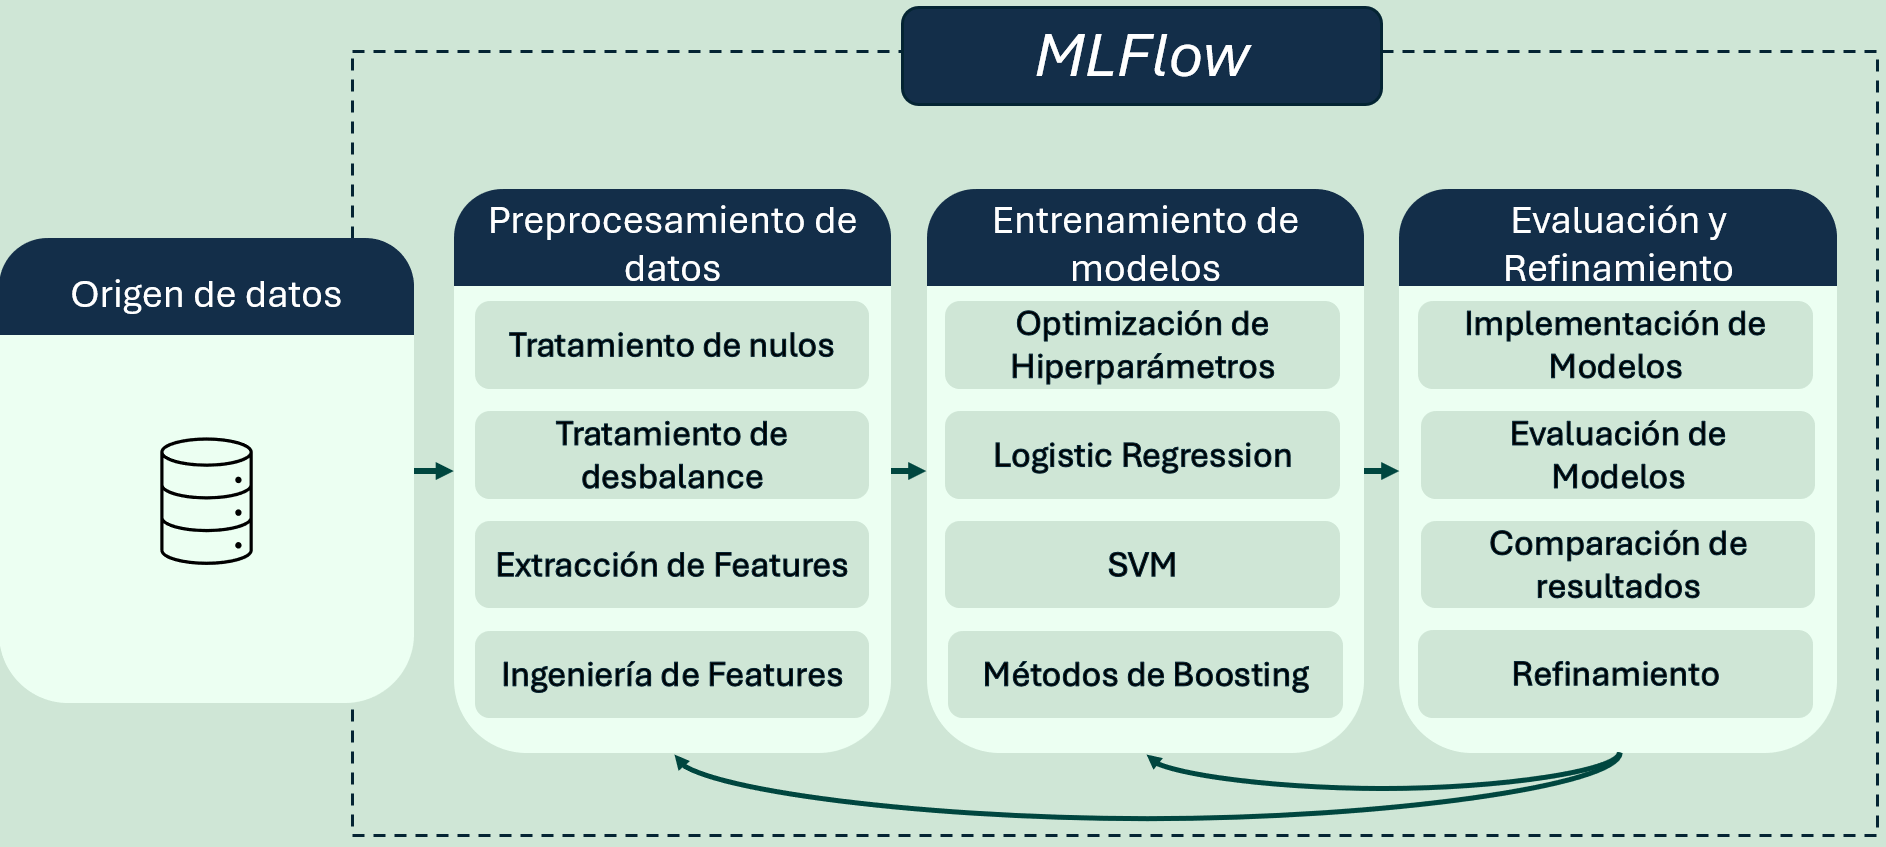
\includegraphics[width=.65\textwidth]{./Figuras/diagrama_bloques.png}
\caption{Diagrama en bloques del sistema.}
\label{fig:diagBloques}
\end{figure}

\vspace{25px}
%\end{consigna} % ELIMINAR \begin{consigna}{red} y \end{consigna}{red} en las secciones que vayan completando para cada entrega parcial.

\section{2. Identificación y análisis de los interesados}
\label{sec:interesados}

\begin{table}[ht]
%\caption{Identificación de los interesados}
%\label{tab:interesados}
\begin{tabularx}{\linewidth}{@{}|l|X|X|l|@{}}
\hline
\rowcolor[HTML]{C0C0C0} 
Rol           & Nombre y Apellido & Organización 	& Puesto 	\\ \hline
Responsable   & \authorname       & FIUBA        	& Alumno 	\\ \hline
Orientador    & \supname	      & \pertesupname 	& Director del Trabajo Final \\ \hline
Usuario final & Mercado financiero                   & -             	& -       	\\ \hline
\end{tabularx}
\end{table}

\begin{itemize}
	\item Orientador: podrán ayudar en la recomendación y evaluación de técnicas a explorar en las diferentes etapas del proyecto.
	\item Usuario final: si bien es un proyecto personal, se considerarán como potenciales usuarios finales a empresas del sector financiero. Estas podrán encontrar interés y utilidad en las predicciones de los modelos explorados.
\end{itemize}

\section{3. Propósito del proyecto}
\label{sec:proposito}

Predecir si una empresa puede entrar en quiebra o no, al explorar técnicas de \textit{machine learning} en un marco de trabajo productivo, reproducible y escalable.

\section{4. Alcance del proyecto}
\label{sec:alcance}

El alcance del proyecto incluye:
\begin{itemize}
	\item Análisis exploratorio de datos: se analizarán las distintas variables presentes en el \textit{dataset} de estudio, con el fin de conocer sus características y poder tomar decisiones en base a ellas.
    \item Preprocesamiento de datos: se realizarán técnicas de tratamiento de datos faltantes, selección y/o extracción de features, como así también de ingeniería de features.
    \item Implementación de modelos de \textit{machine learning}: se estudiarán diversos modelos de aprendizaje de máquina sobre los datos procesados, tales como \textit{logistic regression}, \textit{SVM} y \textit{XGBoost}. Además, se optimizarán los hiperparámetros de estos modelos mediante búsqueda bayesiana.
    \item Evaluación y comparación de modelos: se obtendrán métricas relacionadas a los modelos explorados, con el fin de poder determinar cual de ellos realiza una mejor predicción.
    \item Implementación de un entorno basado en \textit{MLFlow}: este entornó facilitará la realización, la reproducibilidad y la escalabilidad de las distintas etapas de trabajo que se realizarán en este proyecto. El mismo será de caracter local, es decir, no se implementará en una plataforma de \textit{cloud computing}.
\end{itemize}

No se incluye:
\begin{itemize}
    \item El despliegue del entorno de trabajo en una plataforma de \textit{cloud computing}, tales como \textit{Azure}, \textit{AWS}, entre otros.
    \item El análisis de otros \textit{datasets} distintos al propuesto.
\end{itemize}

\section{5. Supuestos del proyecto}
\label{sec:supuestos}

Para el desarrollo del presente proyecto se supone que:
\begin{itemize}
	\item Supuesto 1: el \textit{dataset} de estudio presenta datos fiables, y no tiene restricciones en cuanto a licencias de uso.
	\item Supuesto 2: una \textit{laptop} como equipo de trabajo es más que suficiente para realizar el preprocesamiento y entrenamiento de los modelos de aprendizaje automático.
	\item Supuesto 3: el entorno de \textit{MLFlow} podrá desarrollarse en etapas futuras del proyecto, posteriores a la exploración de los modelos de aprendizaje automático.
    \item Supuesto 4: el entorno de \textit{MLFlow} podrá desplegarse de manera local, sin necesidad de recurrir a plataforma de \textit{cloud computing}, tales como \textit{Azure}, \textit{AWS}, entre otros.
    \item Supuesto 5: se disponen de al menos 15 horas semanales para realizar el proyecto.
\end{itemize}

\section{6. Product Backlog}
\label{sec:backlog}
\textbf{Roles}
\begin{itemize}
    \item \textit{Ingeniero del proyecto}: es quien se encarga del análisis, diseño, desarrollo y despliegue del proyecto.
    \item \textit{Usuario final}: es quien consulta y analiza las predicciones de los modelos explorados en el proyecto.
\end{itemize}

\textbf{Criterios de ponderación de historias de usuario}

Esto son los criterios que se utilizan para ponderar a las historias de usuario mediante \textit{Story Points}:
\begin{itemize}
    \item Dificultad: representa la cantidad de trabajo estimado que requiere la historia de usuario para realizarse.
    \item Complejidad: representa la dificultad de realizar la historia de usuario a nivel técnico.
    \item Incertidumbre: representa el riesgo asociado a la historia de usuario.
\end{itemize}

Cada criterio tiene asociado las ponderaciones \textit{baja}, \textit{media} y \textit{alta}, las cuales se detallan en el cuadro \ref{table:ponderaciones}. Los \textit{Story Points} de una historia de usuario quedan definidos por la suma de los valores de estas ponderaciones redondeada hacia el número superior más próximo en la serie de \textit{Fibonacci}.

\begin{table}[htpb]
\centering
\begin{tabular}{|c|c|c|c|}
\hline
\rowcolor[HTML]{C0C0C0}
Criterio\textbackslash Ponderación & Baja & Media & Alta \\ \hline
Dificultad & 1 & 3 & 5 \\ \hline
Complejidad & 1 & 3 & 5 \\ \hline
Incertidumbre & 1 & 5 & 8 \\ \hline
\end{tabular}
\caption{Tabla de ponderaciones de historia de usuario.}
\label{table:ponderaciones}
\end{table}

\textbf{\'{E}picas}
\begin{itemize}
  \item \textbf{\'{E}pica 1 - Análisis y procesamiento de datos}
    \begin{itemize}
      \item HU1 - Análisis exploratorio
        \begin{itemize}
            \item Como ingeniero del proyecto, quiero realizar un análisis exploratorio de datos para conocer las distribuciones, formas y otras particularidades de las variables del dataset con el que se trabajará.
            \item Ponderación
            \begin{itemize}
                \item Dificultad: Media - 3 \textit{Story Points}
                \item Complejidad: Baja - 1 \textit{Story Points}
                \item Incertidumbre: Baja - 1 \textit{Story Points}
                \item Suma: 5
                \item Total: 5 \textit{Story Points}
            \end{itemize}            
        \end{itemize}
      \item HU2 - Procesamiento de datos faltantes y datos atípicos
        \begin{itemize}
            \item Como ingeniero del proyecto, quiero realizar un procesamiento de datos faltantes y de datos atípicos con el fin de asegurar la calidad del dataset.
            \item Ponderación
            \begin{itemize}
                \item Dificultad: Media - 3 \textit{Story Points}
                \item Complejidad: Media - 3 \textit{Story Points}
                \item Incertidumbre: Baja - 1 \textit{Story Points}
                \item Suma: 7
                \item Total: 8 \textit{Story Points}
            \end{itemize}
        \end{itemize}
      \item HU3 - \textit{Feature Engineering}
        \begin{itemize}
            \item Como ingeniero del proyecto, quiero implementar \textit{Feature Engineering} con el fin de crear nuevos atributos en el dataset.
            \item Ponderación
            \begin{itemize}
                \item Dificultad: Media - 3 \textit{Story Points}
                \item Complejidad: Media - 3 \textit{Story Points}
                \item Incertidumbre: Baja - 1 \textit{Story Points}
                \item Suma: 7 
                \item Total: 8 \textit{Story Points}
            \end{itemize}
        \end{itemize}
    \end{itemize}
  \item \textbf{\'{E}pica 2 - Implementación y comparación de modelos}
    \begin{itemize}
      \item HU4 - Implementación de modelos de \textit{Machine Learning}
        \begin{itemize}
            \item Como ingeniero del proyecto, quiero implementar distintos modelos de \textit{Machine Learning} que permitan predecir si una empresa entra en quiebra o no.
            \item Ponderación
            \begin{itemize}
                \item Dificultad: Media - 3 \textit{Story Points}
                \item Complejidad: Media - 3 \textit{Story Points}
                \item Incertidumbre: Media - 5 \textit{Story Points}
                \item Suma: 11
                \item Total: 13 \textit{Story Points}
            \end{itemize}
        \end{itemize}
      \item HU5 - Optimización de hiperparámetros
        \begin{itemize}
            \item Como ingeniero del proyecto, quiero implementar técnicas de optimización de hiperparámetros y aplicarlas a los modelos de \textit{Machine Learning} implementados.
            \item Ponderación
            \begin{itemize}
                \item Dificultad: Media - 3 \textit{Story Points}
                \item Complejidad: Media - 3 \textit{Story Points}
                \item Incertidumbre: Media - 5 \textit{Story Points}
                \item Suma: 11
                \item Total: 13 \textit{Story Points}
            \end{itemize}
        \end{itemize}
      \item HU6 - Métricas de modelos
        \begin{itemize}
            \item Como ingeniero del proyecto, quiero calcular métricas en cada modelo de \textit{Machine Learning} implementado y comparar sus resultados.
            \item Ponderación
            \begin{itemize}
                \item Dificultad: Media - 3 \textit{Story Points}
                \item Complejidad: Media - 3 \textit{Story Points}
                \item Incertidumbre: Baja - 1 \textit{Story Points}
                \item Suma: 7
                \item Total: 8 \textit{Story Points}
            \end{itemize}
        \end{itemize}
    \end{itemize}
  \item \textbf{\'{E}pica 3 - Despliegue en entorno \textit{MLFlow}}
    \begin{itemize}
      \item HU7 - Despliegue en \textit{MLFlow}
        \begin{itemize}
            \item Como ingeniero del proyecto, quiero desplegar un entorno local de \textit{MLFLow} en donde se repliquen los pasos de procesamiento de datos e implementación y comparación de modelos.
            \item Ponderación
            \begin{itemize}
                \item Dificultad: Alta - 5 \textit{Story Points}
                \item Complejidad: Media - 3 \textit{Story Points}
                \item Incertidumbre: Media - 5 \textit{Story Points}
                \item Suma: 13
                \item Total: 13 \textit{Story Points}
            \end{itemize}
        \end{itemize}
      \item HU8 - \textit{API} para entorno \textit{MLFlow}
        \begin{itemize}
            \item Como ingeniero del proyecto, quiero exponer el entorno de \textit{MLFlow} mediante una \textit{API} para facilitar el acceso y el consumo del mismo.
            \item Ponderación
            \begin{itemize}
                \item Dificultad: Baja - 1 \textit{Story Points}
                \item Complejidad: Media - 3 \textit{Story Points}
                \item Incertidumbre: Baja - 1 \textit{Story Points}
                \item Suma: 5
                \item Total: 5 \textit{Story Points}
            \end{itemize}
        \end{itemize}
    \end{itemize}
  \item \textbf{\'{E}pica 4 - Documentación y calidad}
    \begin{itemize}
      \item HU9 - Implementación de buenas prácticas
        \begin{itemize}
            \item Como ingeniero del proyecto, quiero asegurar que el código siga las buenas prácticas y estándares de la industria.
            \item Ponderación
            \begin{itemize}
                \item Dificultad: Media - 3 \textit{Story Points}
                \item Complejidad: Baja - 1 \textit{Story Points}
                \item Incertidumbre: Baja - 1 \textit{Story Points}
                \item Suma: 5
                \item Total: 5 \textit{Story Points}
            \end{itemize}
        \end{itemize}
      \item HU10 - Documentación
        \begin{itemize}
            \item Como ingeniero del proyecto, quiero documentar todos los pasos realizados durante el proyecto.
            \item Ponderación
            \begin{itemize}
                \item Dificultad: Baja - 1 \textit{Story Points}
                \item Complejidad: Baja - 1 \textit{Story Points}
                \item Incertidumbre: Baja - 1 \textit{Story Points}
                \item Suma: 3
                \item Total: 3 \textit{Story Points}
            \end{itemize}
        \end{itemize}
      \item HU11 - Validación de \textit{API} de \textit{MLFlow}
        \begin{itemize}
            \item Como usuario final, quiero consultar los resultados y comparaciones de los modelos mediante la \textit{API} del entorno de \textbf{MLFlow}, para poder analizarlos.
            \item Ponderación
            \begin{itemize}
                \item Dificultad: Media - 3 \textit{Story Points}
                \item Complejidad: Baja - 1 \textit{Story Points}
                \item Incertidumbre: Baja - 1 \textit{Story Points}
                \item Suma: 5
                \item Total: 5 \textit{Story Points}
            \end{itemize}
        \end{itemize}        
    \end{itemize}
\end{itemize}

\section{7. Criterios de aceptación de historias de usuario}
\label{sec:criteriosAceptacion}

\begin{itemize}
  \item \textbf{\'{E}pica 1 - Análisis y procesamiento de datos}
    \begin{itemize}
      \item Criterios de aceptación HU1 - Análisis exploratorio
        \begin{itemize}
            \item Se estudia la presencia de datos atípicos y de datos faltantes para cada variable.
            \item Se grafican las distribuciones de las variables del dataset.
            \item Se realiza un estudio de correlaciones entre variables numéricas.
            \item Se documentan los hallazgos del análisis de cada variable.
        \end{itemize}
      \item Criterios de aceptación HU2 - Procesamiento de datos faltantes y datos atípicos
        \begin{itemize}
            \item Se realiza una imputación de datos faltantes a las variables del dataset.
            \item Se justifican los métodos de imputación utilizados.
            \item Se ajustan los datos atípicos de las variables del dataset.
            \item Se justifican los métodos de ajuste utilizados.
            \item Se justifican los casos en donde se decide no imputar ni ajustar.
        \end{itemize}
      \item Criterios de aceptación HU3 - \textit{Feature Engineering}
        \begin{itemize}
            \item Se crean nuevas variables en el dataset a partir de las existentes.
            \item Se estudia el impacto por separado de estas variables en los modelos generados, a partir de sus métricas.
            \item Se justifica la inclusión o no en el modelo de cada variable generada.
        \end{itemize}
    \end{itemize}
  \item \textbf{\'{E}pica 2 - Implementación y comparación de modelos}
    \begin{itemize}
      \item Criterios de aceptación HU4 - Implementación de modelos de \textit{Machine Learning}
        \begin{itemize}
            \item Se implementan distintos modelos de \textit{Machine Learning}.
            \item Se justifica el uso de cada uno de los modelos implementados.
            \item Se persisten los modelos generados en GitHub, para futuros análisis y comparaciones.
        \end{itemize}
      \item Criterios de aceptación HU5 - Optimización de hiperparámetros
        \begin{itemize}
            \item Se seleccionan los hiperparámetros de cada modelo a optimizar.
            \item Se define el rango sobre el cual se optimizará cada hiperparámetro.
            \item Se realiza una búsqueda del valor óptimo de los hiperparámetros en los rangos definidos.
            \item Se justifican las decisiones tomadas en cada paso.
        \end{itemize}
      \item Criterios de aceptación HU6 - Métricas de modelos
        \begin{itemize}
            \item Se definen las métricas de análisis para cada modelo.
            \item Se justifica la selección de cada métrica para cada modelo.
            \item Se obtienen las métricas de análisis de cada modelo.
            \item Se comparan los distintos modelos mediante las métricas definidas.
        \end{itemize}
    \end{itemize}
  \item \textbf{\'{E}pica 3 - Despliegue en entorno \textit{MLFlow}}
    \begin{itemize}
      \item Criterios de aceptación HU7 - Despliegue en \textit{MLFlow}
        \begin{itemize}
            \item Se crea un entorno \textit{MLFlow} local desde cero
            \item Se configura el paso correspondiente al análisis de datos en el entorno.
            \item Se replican las técnicas exploradas de análisis de datos en el paso correspondiente.
            \item Se configura el paso de entrenamiento de modelos en el entorno.
            \item Se replican las técnicas exploradas de entrenamiento  de modelos en el paso correspondiente.
            \item Se configura el paso de evaluación de modelos en el entorno.
            \item Se replican las técnicas exploradas de evaluación de modelos en el paso correspondiente.
        \end{itemize}
      \item Criterios de aceptación HU8 - \textit{API} para entorno \textit{MLFlow}
        \begin{itemize}
            \item Se exponen los resultados de los modelos explorados en el entorno de \textit{MLFlow} mediante una \textit{API}.
            \item Se exponen las comparaciones de los modelos explorados en el entorno de \textit{MLFlow} mediante una \textit{API}.
        \end{itemize}
    \end{itemize}
  \item \textbf{\'{E}pica 4 - Documentación y calidad}
    \begin{itemize}
      \item Criterios de aceptación HU9 - Implementación de buenas prácticas
        \begin{itemize}
            \item Se implementan buenas prácticas de código \textit{Python} en el proyecto.
        \end{itemize}
      \item Criterios de aceptación HU10 - Documentación
        \begin{itemize}
            \item Se documentan todos los pasos realizados durante el desarrollo del proyecto.
            \item Se valida que cada paso realizado esté correctamente justificado.
        \end{itemize}
      \item Criterios de aceptación HU11 - Validación de \textit{API} de \textit{MLFlow}
        \begin{itemize}
            \item Se valida el acceso a los resultados de los modelos mediante la \textit{API} del entorno \textit{MLFlow}.
            \item Se valida el acceso a la comparación de los modelos mediante la \textit{API} del entorno \textit{MLFlow}.
        \end{itemize}
    \end{itemize}
\end{itemize}

\section{8. Fases de CRISP-DM}

\begin{enumerate}
  \item \textbf{Comprensión del negocio:}
    \begin{itemize}
        \item \textit{Objetivo:} predecir si una empresa va a entrar en quiebra o no.
        \item \textit{Impacto:} ayudar en la toma de decisiones a empresas especializadas en finanzas, en inversiones, en prestación de seguros, entre otras, permitiéndoles saber si una empresa sobre la cual se quiere invertir o a la cual se le quiere otorgar un préstamo puede entrar en quiebra o no.
        \item \textit{Métricas:} se predice correctamente si la empresa quiebra o no.
    \end{itemize}
  \item \textbf{Comprensión de los datos}
    \begin{itemize}
        \item \textit{Tipos de datos:} datos tabulares.
        \item \textit{Fuente de datos:} datos publicados por el \href{https://www.tejwin.com/en/}{Taiwan Economic Journal}.
        \item \textit{Cantidad de datos:} 6819 registros con 96 columnas.
    \end{itemize}
  \item \textbf{Preparación de los datos}
    \begin{itemize}
        \item \textit{Transformaciones}
            \begin{itemize}
                \item Análisis y ajuste de datos atípicos.
                \item Análisis y ajuste de datos faltantes.
                \item Creación de nuevas variables al combinar las variables existentes.
                \item Normalización de datos.
            \end{itemize}
        \item \textit{Características clave}
            \begin{itemize}
                \item Indicador de si la empresa entró en quiebra o variable \textit{target}.
                \item Distintas métricas del desempeño de la empresa a nivel económico y contable.
            \end{itemize}
    \end{itemize}
  \item \textbf{Modelado}
    \begin{itemize}
        \item \textit{Tipo de problema:} Clasificación.
        \item \textit{Arquitecturas posibles:} Modelos de clasificación como \textit{Logistic Regression}, \textit{Support Vector Machines} y \textit{XGBoost}.
    \end{itemize}
  \item \textbf{Evaluación del modelo}
    \begin{itemize}
        \item \textit{F1-score} y \textit{AUC-ROC}.
    \end{itemize}
  \item \textbf{Despliegue del modelo}
    \begin{itemize}
        \item Despliegue local usando \textit{MLFlow}.
    \end{itemize}
\end{enumerate}

\section{9. Desglose del trabajo en tareas}
\label{sec:wbs}

\begin{itemize}
    \item HU1 - Análisis exploratorio (21 h).
        \begin{itemize}
            \item Identificar variables \textit{categóricas}.
                \begin{itemize}
                    \item \textit{Estimación:} 4 h.
                    \item \textit{Prioridad:} Media.
                \end{itemize}
            \item Identificar variables \textit{numéricas}.
                \begin{itemize}
                    \item \textit{Estimación:} 4 h.
                    \item \textit{Prioridad:} Media.
                \end{itemize}
            \item Graficar la distribución de las variables \textit{numéricas}.
                \begin{itemize}
                    \item \textit{Estimación:} 6 h.
                    \item \textit{Prioridad:} Media.
                \end{itemize}
            \item Realizar análisis de correlaciones entre variables \textit{numéricas}.
                \begin{itemize}
                    \item \textit{Estimación:} 4 h.
                    \item \textit{Prioridad:} Media.
                \end{itemize}
            \item Documentar pasos y decisiones tomadas.
                \begin{itemize}
                    \item \textit{Estimación:} 3 h.
                    \item \textit{Prioridad:} Media.
                \end{itemize}
        \end{itemize}
    \item HU2 - Procesamiento de datos faltantes y datos atípicos (64 h).
        \begin{itemize}
            \item Investigar técnicas de balanceo de clases para algoritmos de clasificación.
                \begin{itemize}
                    \item \textit{Estimación:} 6 h.
                    \item \textit{Prioridad:} Media.
                \end{itemize}
            \item Implementar técnicas de balanceo de clases para algoritmos de clasificación.
                \begin{itemize}
                    \item \textit{Estimación:} 5 h.
                    \item \textit{Prioridad:} Media.
                \end{itemize}
            \item Separar \textit{dataset} en \textit{train} y \textit{test}.
                \begin{itemize}
                    \item \textit{Estimación:} 3 h.
                    \item \textit{Prioridad:} Media.
                \end{itemize}
            \item Identificar variables con datos faltantes.
                \begin{itemize}
                    \item \textit{Estimación:} 4 h.
                    \item \textit{Prioridad:} Alta.
                \end{itemize}
            \item Analizar causas de datos faltantes.
                \begin{itemize}
                    \item \textit{Estimación:} 6 h.
                    \item \textit{Prioridad:} Alta.
                \end{itemize}
            \item Corregir datos faltantes.
                \begin{itemize}
                    \item \textit{Estimación:} 8 h.
                    \item \textit{Prioridad:} Alta.
                \end{itemize}
            \item Identificar datos con valores atípicos.
                \begin{itemize}
                    \item \textit{Estimación:} 6 h.
                    \item \textit{Prioridad:} Alta.
                \end{itemize}
            \item Analizar causas de datos atípicos.
                \begin{itemize}
                    \item \textit{Estimación:} 8 h.
                    \item \textit{Prioridad:} Alta.
                \end{itemize}
            \item Graficar variables que presentan de datos atípicos.
                \begin{itemize}
                    \item \textit{Estimación:} 5 h.
                    \item \textit{Prioridad:} Media.
                \end{itemize}
            \item Corregir datos atípicos.
                \begin{itemize}
                    \item \textit{Estimación:} 8 h.
                    \item \textit{Prioridad:} Alta.
                \end{itemize}
            \item Documentar pasos y decisiones tomadas.
                \begin{itemize}
                    \item \textit{Estimación:} 5 h.
                    \item \textit{Prioridad:} Media.
                \end{itemize}
        \end{itemize}
    \item HU3 - \textit{Feature Engineering} (38 h).
        \begin{itemize}
            \item Identificar variables menos importantes para eliminarlas.
                \begin{itemize}
                    \item \textit{Estimación:} 5 h.
                    \item \textit{Prioridad:} Alta.
                \end{itemize}
            \item Implementar técnicas de eliminación de features.
                \begin{itemize}
                    \item \textit{Estimación:} 5 h.
                    \item \textit{Prioridad:} Media.
                \end{itemize}
            \item Crear nuevas variables mediante combinaciones lineales de variables existentes.
                \begin{itemize}
                    \item \textit{Estimación:} 7 h.
                    \item \textit{Prioridad:} Alta.
                \end{itemize}
            \item Investigar otras técnicas de creación de variables.
                \begin{itemize}
                    \item \textit{Estimación:} 5 h.
                    \item \textit{Prioridad:} Media.
                \end{itemize}
            \item Aplicar otras técnicas de creación de variables.
                \begin{itemize}
                    \item \textit{Estimación:} 8 h.
                    \item \textit{Prioridad:} Alta.
                \end{itemize}
            \item Evaluar nuevas variables en modelos.
                \begin{itemize}
                    \item \textit{Estimación:} 5 h.
                    \item \textit{Prioridad:} Alta.
                \end{itemize}
            \item Documentar pasos y decisiones tomadas.
                \begin{itemize}
                    \item \textit{Estimación:} 3 h.
                    \item \textit{Prioridad:} Baja.
                \end{itemize}
        \end{itemize}
    \item HU4 - Implementación de modelos de \textit{Machine Learning} (89 h).
        \begin{itemize}
            \item Implementar código de validación cruzada para \textit{Logistic Regression}.
                \begin{itemize}
                    \item \textit{Estimación:} 4 h.
                    \item \textit{Prioridad:} Media.
                \end{itemize}
            \item Implementar modelo \textit{Logistic Regression}, sin considerar \textit{feature engineering}.
                \begin{itemize}
                    \item \textit{Estimación:} 6 h.
                    \item \textit{Prioridad:} Alta.
                \end{itemize}
            \item Evaluar modelo \textit{Logistic Regression}, sin considerar \textit{feature engineering}.
                \begin{itemize}
                    \item \textit{Estimación:} 4 h.
                    \item \textit{Prioridad:} Media.
                \end{itemize}
            \item Implementar modelo \textit{Logistic Regression}, considerando \textit{feature engineering}.
                \begin{itemize}
                    \item \textit{Estimación:} 6 h.
                    \item \textit{Prioridad:} Alta.
                \end{itemize}
            \item Evaluar modelo \textit{Logistic Regression}, considerando \textit{feature engineering}.
                \begin{itemize}
                    \item \textit{Estimación:} 4 h.
                    \item \textit{Prioridad:} Media.
                \end{itemize}
            \item Implementar código de validación cruzada para \textit{SVM}.
                \begin{itemize}
                    \item \textit{Estimación:} 4 h.
                    \item \textit{Prioridad:} Media.
                \end{itemize}
            \item Implementar modelo \textit{SVM}, sin considerar \textit{feature engineering}.
                \begin{itemize}
                    \item \textit{Estimación:} 6 h.
                    \item \textit{Prioridad:} Alta.
                \end{itemize}
            \item Evaluar modelo \textit{SVM}, sin considerar \textit{feature engineering}.
                \begin{itemize}
                    \item \textit{Estimación:} 4 h.
                    \item \textit{Prioridad:} Media.
                \end{itemize}
            \item Implementar modelo \textit{SVM}, considerando \textit{feature engineering}.
                \begin{itemize}
                    \item \textit{Estimación:} 6 h.
                    \item \textit{Prioridad:} Alta.
                \end{itemize}
            \item Evaluar modelo \textit{SVM}, considerando \textit{feature engineering}.
                \begin{itemize}
                    \item \textit{Estimación:} 4 h.
                    \item \textit{Prioridad:} Media.
                \end{itemize}
            \item Implementar código de validación cruzada para \textit{XGBoost}.
                \begin{itemize}
                    \item \textit{Estimación:} 4 h.
                    \item \textit{Prioridad:} Media.
                \end{itemize}
            \item Implementar modelo \textit{XGBoost}, sin considerar \textit{feature engineering}.
                \begin{itemize}
                    \item \textit{Estimación:} 8 h.
                    \item \textit{Prioridad:} Alta.
                \end{itemize}
            \item Evaluar modelo \textit{XGBoost}, sin considerar \textit{feature engineering}.
                \begin{itemize}
                    \item \textit{Estimación:} 6 h.
                    \item \textit{Prioridad:} Media.
                \end{itemize}
            \item Implementar modelo \textit{XGBoost}, considerando \textit{feature engineering}.
                \begin{itemize}
                    \item \textit{Estimación:} 8 h.
                    \item \textit{Prioridad:} Alta.
                \end{itemize}
            \item Evaluar modelo \textit{XGBoost}, considerando \textit{feature engineering}.
                \begin{itemize}
                    \item \textit{Estimación:} 6 h.
                    \item \textit{Prioridad:} Media.
                \end{itemize}
            \item Persistir modelos en \textit{GitHub}
                \begin{itemize}
                    \item \textit{Estimación:} 4 h
                    \item \textit{Prioridad:} Media
                \end{itemize}
            \item Documentar pasos y decisiones tomadas.
                \begin{itemize}
                    \item \textit{Estimación:} 5 h.
                    \item \textit{Prioridad:} Media.
                \end{itemize}
        \end{itemize}
    \item HU5 - Optimización de hiperparámetros (118 h).
        \begin{itemize}
            \item Identificar hiperparámetros y rangos de \textit{Logistic Regression}.
                \begin{itemize}
                    \item \textit{Estimación:} 5 h.
                    \item \textit{Prioridad:} Media.
                \end{itemize}
            \item Optimizar hiperparámetros de \textit{Logistic Regression}, sin considerar \textit{feature engineering}.
                \begin{itemize}
                    \item \textit{Estimación:} 6 h.
                    \item \textit{Prioridad:} Media.
                \end{itemize}
            \item Implementar hiperparámetros más óptimos en \textit{Logistic Regression}, sin considerar \textit{feature engineering}.
                \begin{itemize}
                    \item \textit{Estimación:} 4 h.
                    \item \textit{Prioridad:} Media.
                \end{itemize}
            \item Evaluar modelo de \textit{Logistic Regression} con hiperparámetros óptimos, sin considerar \textit{feature engineering}.
                \begin{itemize}
                    \item \textit{Estimación:} 4 h.
                    \item \textit{Prioridad:} Media.
                \end{itemize}
            \item Optimizar hiperparámetros de \textit{Logistic Regression}, considerando \textit{feature engineering}.
                \begin{itemize}
                    \item \textit{Estimación:} 6 h.
                    \item \textit{Prioridad:} Media.
                \end{itemize}
            \item Implementar hiperparámetros más óptimos en \textit{Logistic Regression}, considerando \textit{feature engineering}.
                \begin{itemize}
                    \item \textit{Estimación:} 4 h.
                    \item \textit{Prioridad:} Media.
                \end{itemize}
            \item Evaluar modelo de \textit{Logistic Regression} con hiperparámetros óptimos, considerando \textit{feature engineering}.
                \begin{itemize}
                    \item \textit{Estimación:} 4 h.
                    \item \textit{Prioridad:} Media.
                \end{itemize}            
            \item Identificar hiperparámetros y rangos de \textit{SVM}.
                \begin{itemize}
                    \item \textit{Estimación:} 5 h.
                    \item \textit{Prioridad:} Media.
                \end{itemize}
            \item Optimizar hiperparámetros de \textit{SVM}, sin considerar \textit{feature engineering}.
                \begin{itemize}
                    \item \textit{Estimación:} 6 h.
                    \item \textit{Prioridad:} Media.
                \end{itemize}
            \item Implementar hiperparámetros más óptimos en \textit{SVM}, sin considerar \textit{feature engineering}.
                \begin{itemize}
                    \item \textit{Estimación:} 4 h.
                    \item \textit{Prioridad:} Media.
                \end{itemize}
            \item Evaluar modelo de \textit{SVM} con hiperparámetros óptimos, sin considerar \textit{feature engineering}.
                \begin{itemize}
                    \item \textit{Estimación:} 4 h.
                    \item \textit{Prioridad:} Media.
                \end{itemize}
            \item Optimizar hiperparámetros de \textit{SVM}, considerando \textit{feature engineering}.
                \begin{itemize}
                    \item \textit{Estimación:} 6 h.
                    \item \textit{Prioridad:} Media.
                \end{itemize}
            \item Implementar hiperparámetros más óptimos en \textit{SVM}, considerando \textit{feature engineering}.
                \begin{itemize}
                    \item \textit{Estimación:} 4 h.
                    \item \textit{Prioridad:} Media.
                \end{itemize}
            \item Evaluar modelo de \textit{SVM} con hiperparámetros óptimos, considerando \textit{feature engineering}.
                \begin{itemize}
                    \item \textit{Estimación:} 4 h.
                    \item \textit{Prioridad:} Media.
                \end{itemize}           
            \item Identificar hiperparámetros y rangos de \textit{XGBoost}.
                \begin{itemize}
                    \item \textit{Estimación:} 7 h.
                    \item \textit{Prioridad:} Media.
                \end{itemize}
            \item Optimizar hiperparámetros de \textit{XGBoost}, sin considerar \textit{feature engineering}.
                \begin{itemize}
                    \item \textit{Estimación:} 8 h.
                    \item \textit{Prioridad:} Alta.
                \end{itemize}
            \item Implementar hiperparámetros más óptimos en \textit{XGBoost}, sin considerar \textit{feature engineering}.
                \begin{itemize}
                    \item \textit{Estimación:} 5 h.
                    \item \textit{Prioridad:} Media.
                \end{itemize}
            \item Evaluar modelo de \textit{XGBoost} con hiperparámetros óptimos, sin considerar \textit{feature engineering}.
                \begin{itemize}
                    \item \textit{Estimación:} 7 h.
                    \item \textit{Prioridad:} Media.
                \end{itemize}
            \item Optimizar hiperparámetros de \textit{XGBoost}, considerando \textit{feature engineering}.
                \begin{itemize}
                    \item \textit{Estimación:} 8 h.
                    \item \textit{Prioridad:} Alta.
                \end{itemize}
            \item Implementar hiperparámetros más óptimos en \textit{XGBoost}, considerando \textit{feature engineering}.
                \begin{itemize}
                    \item \textit{Estimación:} 5 h.
                    \item \textit{Prioridad:} Media.
                \end{itemize}
            \item Evaluar modelo de \textit{XGBoost} con hiperparámetros óptimos, considerando \textit{feature engineering}.
                \begin{itemize}
                    \item \textit{Estimación:} 7 h.
                    \item \textit{Prioridad:} Media.
                \end{itemize}  
            \item Documentar pasos y decisiones tomadas.
                \begin{itemize}
                    \item \textit{Estimación:} 5 h.
                    \item \textit{Prioridad:} Media.
                \end{itemize}
        \end{itemize}
    \item HU6 - Métricas de modelos (56 h).
        \begin{itemize}
            \item Obtener métricas de \textit{F1-score} para \textit{Logistic Regression}, sin  considerar \textit{feature engineering}.
                \begin{itemize}
                    \item \textit{Estimación:} 3 h.
                    \item \textit{Prioridad:} Media.
                \end{itemize}
            \item Obtener métricas de \textit{AUC-ROC} para \textit{Logistic Regression}, sin  considerar \textit{feature engineering}, y graficar.
                \begin{itemize}
                    \item \textit{Estimación:} 5 h.
                    \item \textit{Prioridad:} Media.
                \end{itemize}
            \item Obtener métricas de \textit{F1-score} para \textit{Logistic Regression}, considerando \textit{feature engineering}.
                \begin{itemize}
                    \item \textit{Estimación:} 3 h.
                    \item \textit{Prioridad:} Media.
                \end{itemize}
            \item Obtener métricas de \textit{AUC-ROC} para \textit{Logistic Regression}, considerando \textit{feature engineering}, y graficar.
                \begin{itemize}
                    \item \textit{Estimación:} 5 h.
                    \item \textit{Prioridad:} Media.
                \end{itemize}                
            \item Obtener métricas de \textit{F1-score} para \textit{SVM}, sin  considerar \textit{feature engineering}.
                \begin{itemize}
                    \item \textit{Estimación:} 3 h.
                    \item \textit{Prioridad:} Media.
                \end{itemize}
            \item Obtener métricas de \textit{AUC-ROC} para \textit{SVM}, sin  considerar \textit{feature engineering}, y graficar.
                \begin{itemize}
                    \item \textit{Estimación:} 5 h.
                    \item \textit{Prioridad:} Media.
                \end{itemize}
            \item Obtener métricas de \textit{F1-score} para \textit{SVM}, considerando \textit{feature engineering}.
                \begin{itemize}
                    \item \textit{Estimación:} 3 h.
                    \item \textit{Prioridad:} Media.
                \end{itemize}
            \item Obtener métricas de \textit{AUC-ROC} para \textit{SVM}, considerando \textit{feature engineering}, y graficar.
                \begin{itemize}
                    \item \textit{Estimación:} 5 h.
                    \item \textit{Prioridad:} Media.
                \end{itemize}                
            \item Obtener métricas de \textit{F1-score} para \textit{XGBoost}, sin  considerar \textit{feature engineering}.
                \begin{itemize}
                    \item \textit{Estimación:} 3 h.
                    \item \textit{Prioridad:} Media.
                \end{itemize}
            \item Obtener métricas de \textit{AUC-ROC} para \textit{XGBoost}, sin  considerar \textit{feature engineering}, y graficar.
                \begin{itemize}
                    \item \textit{Estimación:} 5 h.
                    \item \textit{Prioridad:} Media.
                \end{itemize}
            \item Obtener métricas de \textit{F1-score} para \textit{XGBoost}, considerando \textit{feature engineering}.
                \begin{itemize}
                    \item \textit{Estimación:} 3 h.
                    \item \textit{Prioridad:} Media.
                \end{itemize}
            \item Obtener métricas de \textit{AUC-ROC} para \textit{XGBoost}, considerando \textit{feature engineering}, y graficar.
                \begin{itemize}
                    \item \textit{Estimación:} 5 h.
                    \item \textit{Prioridad:} Media.
                \end{itemize}                
            \item Comparar métricas de distintos modelos.
                \begin{itemize}
                    \item \textit{Estimación:} 3 h.
                    \item \textit{Prioridad:} Media.
                \end{itemize}
            \item Documentar pasos y decisiones tomadas.
                \begin{itemize}
                    \item \textit{Estimación:} 5 h.
                    \item \textit{Prioridad:} Media.
                \end{itemize}
        \end{itemize}
    \item HU7 - Despliegue en \textit{MLFlow} (66 h).
        \begin{itemize}
            \item Investigar buenas prácticas para despliegues de \textit{MLFlow}.
                \begin{itemize}
                    \item \textit{Estimación:} 5 h.
                    \item \textit{Prioridad:} Alta.
                \end{itemize}
            \item Crear entorno local para despliegue \textit{MLFlow}.
                \begin{itemize}
                    \item \textit{Estimación:} 7 h.
                    \item \textit{Prioridad:} Alta.
                \end{itemize}
             \item Replicar técnicas de análisis de datos en entorno \textit{MLFlow}.
                \begin{itemize}
                    \item \textit{Estimación:} 8 h.
                    \item \textit{Prioridad:} Alta.
                \end{itemize}
            \item Replicar técnicas de entrenamiento de modelos de \textit{Logistic Regression} en entorno \textit{MLFlow}.
                \begin{itemize}
                    \item \textit{Estimación:} 8 h.
                    \item \textit{Prioridad:} Alta.
                \end{itemize}
            \item Replicar técnicas de entrenamiento de modelos de \textit{SVM} en entorno \textit{MLFlow}.
                \begin{itemize}
                    \item \textit{Estimación:} 8 h.
                    \item \textit{Prioridad:} Alta.
                \end{itemize}
            \item Replicar técnicas de entrenamiento de modelos de \textit{XGBoost} en entorno \textit{MLFlow}.
                \begin{itemize}
                    \item \textit{Estimación:} 8 h.
                    \item \textit{Prioridad:} Alta.
                \end{itemize}
            \item Replicar técnicas de evaluación de modelos en entorno \textit{MLFlow}.
                \begin{itemize}
                    \item \textit{Estimación:} 8 h.
                    \item \textit{Prioridad:} Alta.
                \end{itemize}
            \item Ejecutar localmente el entorno \textit{MLFlow}.
                \begin{itemize}
                    \item \textit{Estimación:} 4 h.
                    \item \textit{Prioridad:} Media.
                \end{itemize}
            \item Validar ejecución local del entorno \textit{MLFlow}.
                \begin{itemize}
                    \item \textit{Estimación:} 4 h.
                    \item \textit{Prioridad:} Media.
                \end{itemize}
            \item Documentar pasos y decisiones tomadas \textit{MLFlow}.
                \begin{itemize}
                    \item \textit{Estimación:} 6 h.
                    \item \textit{Prioridad:} Media.
                \end{itemize}
        \end{itemize}
    \item HU8 - \textit{API} para entorno \textit{MLFlow} (24 h).
        \begin{itemize}
            \item Investigar como exponer un entorno \textit{MLFlow} mediante \textit{API}.
                \begin{itemize}
                    \item \textit{Estimación:} 5 h.
                    \item \textit{Prioridad:} Media.
                \end{itemize}
            \item Exponer resultados de modelos explorados en entorno \textit{MLFlow} mediante \textit{API}.
                \begin{itemize}
                    \item \textit{Estimación:} 8 h.
                    \item \textit{Prioridad:} Alta.
                \end{itemize}
            \item Exponer comparación de modelos en entorno \textit{MLFlow} mediante \textit{API}.
                \begin{itemize}
                    \item \textit{Estimación:} 8 h.
                    \item \textit{Prioridad:} Alta.
                \end{itemize}
            \item Documentar pasos y decisiones tomadas.
                \begin{itemize}
                    \item \textit{Estimación:} 3 h.
                    \item \textit{Prioridad:} Baja.
                \end{itemize}
        \end{itemize}
    \item HU9 - Implementación de buenas prácticas (12 h).
        \begin{itemize}
            \item Investigar buenas prácticas en código \textit{Python}.
                \begin{itemize}
                    \item \textit{Estimación:} 4 h.
                    \item \textit{Prioridad:} Baja.
                \end{itemize}
            \item Aplicar buenas prácticas en código \textit{Python}.
                \begin{itemize}
                    \item \textit{Estimación:} 8 h.
                    \item \textit{Prioridad:} Media.
                \end{itemize}
        \end{itemize}
    \item HU10 - Documentación (14 h).
        \begin{itemize}
            \item Asegurar que cada decisión tomada haya sido justificada y documentada.
                \begin{itemize}
                    \item \textit{Estimación:} 6 h.
                    \item \textit{Prioridad:} Media.
                \end{itemize}
            \item Asegurar ortografía y formato en documentación.
                \begin{itemize}
                    \item \textit{Estimación:} 8 h.
                    \item \textit{Prioridad:} Media.
                \end{itemize}
        \end{itemize}
    \item HU11 - Validación de \textit{API} de \textit{MLFlow} (21 h).
        \begin{itemize}
            \item Validar acceso a modelos explorados mediante \textit{API} de entorno \textit{MLFlow}.
                \begin{itemize}
                    \item \textit{Estimación:} 8 h.
                    \item \textit{Prioridad:} Media.
                \end{itemize}
            \item Validar acceso a comparación de modelos mediante \textit{API} de entorno \textit{MLFlow}.
                \begin{itemize}
                    \item \textit{Estimación:} 8 h.
                    \item \textit{Prioridad:} Media.
                \end{itemize}
            \item Crear documentación sobre el uso de \textit{API} de entorno \textit{MLFlow}.
                \begin{itemize}
                    \item \textit{Estimación:} 5 h.
                    \item \textit{Prioridad:} Media.
                \end{itemize}
        \end{itemize}
    \item Planificación del proyecto y confección de informes de avance (opcional)(32 h).
        \begin{itemize}
            \item Planificación del proyecto.
                \begin{itemize}
                    \item \textit{Estimación:} 8 h.
                    \item \textit{Prioridad:} Alta.
                \end{itemize}
            \item Informe de avance - Secciones 1 a 5 inclusive.
                \begin{itemize}
                    \item \textit{Estimación:} 6 h.
                    \item \textit{Prioridad:} Media.
                \end{itemize}
            \item Informe de avance - Secciones 6 a 9 inclusive.
                \begin{itemize}
                    \item \textit{Estimación:} 5 h.
                    \item \textit{Prioridad:} Media.
                \end{itemize}
            \item Informe de avance - Secciones 10 a 12 inclusive.
                \begin{itemize}
                    \item \textit{Estimación:} 4 h.
                    \item \textit{Prioridad:} Media.
                \end{itemize}
            \item Informe de avance - Secciones 13 a 15 inclusive.
                \begin{itemize}
                    \item \textit{Estimación:} 4 h.
                    \item \textit{Prioridad:} Media.
                \end{itemize}
            \item Informe de avance - Correciones generales.
                \begin{itemize}
                    \item \textit{Estimación:} 5 h.
                    \item \textit{Prioridad:} Media.
                \end{itemize}
        \end{itemize}   
    \item Redacción de memoria (opcional)(35 h).
        \begin{itemize}
            \item Redacción de sección sobre \textit{procesamiento de datos}.
                \begin{itemize}
                    \item \textit{Estimación:} 6 h.
                    \item \textit{Prioridad:} Media.
                \end{itemize}
            \item Redacción de sección sobre \textit{Feature Engineering}.
                \begin{itemize}
                    \item \textit{Estimación:} 3 h.
                    \item \textit{Prioridad:} Media.
                \end{itemize}
            \item Redacción de sección sobre \textit{implementación de modelos}.
                \begin{itemize}
                    \item \textit{Estimación:} 7 h.
                    \item \textit{Prioridad:} Media.
                \end{itemize}
            \item Redacción de sección sobre \textit{optimización de hiperparámetros}.
                \begin{itemize}
                    \item \textit{Estimación:} 6 h.
                    \item \textit{Prioridad:} Media.
                \end{itemize}
            \item Redacción de sección sobre \textit{MLFlow}.
                \begin{itemize}
                    \item \textit{Estimación:} 5 h.
                    \item \textit{Prioridad:} Media.
                \end{itemize}
            \item Correcciones generales.
                \begin{itemize}
                    \item \textit{Estimación:} 8 h.
                    \item \textit{Prioridad:} Media.
                \end{itemize}
        \end{itemize} 
    \item Preparación de presentación final (opcional)(14 h).
        \begin{itemize}
            \item Confección de presentación \textit{PowerPoint}.
                \begin{itemize}
                    \item \textit{Estimación:} 6 h.
                    \item \textit{Prioridad:} Alta.
                \end{itemize}
            \item Confección de video demostración.
                \begin{itemize}
                    \item \textit{Estimación:} 8 h.
                    \item \textit{Prioridad:} Alta.
                \end{itemize}
        \end{itemize}
\end{itemize}

\section{10. Diagrama de Gantt}
\label{sec:gantt}

El diagrama de Gantt debe representar de forma visual y cronológica todas las tareas del proyecto, abarcando aproximadamente 600 horas totales, de las cuales entre 480 y 500 deben destinarse a tareas técnicas (desarrollo, pruebas, implementación) y entre 100 y 120 a tareas no técnicas (planificación, documentación, escritura de memoria y preparación de la defensa).

\textbf{Consignas y recomendaciones:}
\begin{itemize}
  \item Incluir tanto tareas técnicas derivadas de las HU como tareas no técnicas generales del proyecto.
  \item El eje vertical debe listar las tareas y el eje horizontal representar el tiempo en semanas o fechas.
  \item Utilizar colores diferenciados para distinguir tareas técnicas y no técnicas.
  \item Las tareas deben estar ordenadas cronológicamente y reflejar todo el ciclo del proyecto.
  \item Iniciar con la planificación del proyecto (coincidente con el inicio de Gestión de Proyectos) y finalizar con la defensa, próxima a la fecha de cierre del trabajo.
  \item Configurar el software para mostrar los códigos del desglose de tareas y los nombres junto a cada barra.
  \item Asegurarse de que la fecha final coincida con la del Acta Constitutiva.
  \item Evitar tareas genéricas o ambiguas y asegurar una secuencia lógica y realista.
  \item Las fechas pueden ser aproximadas; ajustar el ancho del diagrama según el texto y el parámetro \texttt{x unit}. Para mejorar la apariencia del diagrama, es necesario ajustar este valor y, quizás, acortar los nombres de las tareas.
\end{itemize}

\textbf{Herramientas sugeridas:}
\begin{itemize}
  \item Planner, GanttProject, Trello + plugins\\
  \url{https://blog.trello.com/es/diagrama-de-gantt-de-un-proyecto}
  \item Creately (colaborativa online)\\
  \url{https://creately.com/diagram/example/ieb3p3ml/LaTeX}
  \item LaTeX con \texttt{pgfgantt}:\\
  \url{http://ctan.dcc.uchile.cl/graphics/pgf/contrib/pgfgantt/pgfgantt.pdf}
\end{itemize}

Incluir una imagen legible del diagrama de Gantt. Si es muy ancho, presentar primero la tabla y luego el gráfico de barras.

\section{11. Planificación de Sprints}

Organizar las tareas técnicas del proyecto en sprints de trabajo que permitan distribuir de forma equilibrada la carga horaria total, estimada en 600 horas.

\textbf{Consigna:}
\begin{itemize}
  \item Completar una tabla que relacione sprints con HU y tareas técnicas correspondientes.
  \item Incluir estimación en horas para cada tarea.
  \item Indicar responsable y porcentaje de avance estimado o completado.
  \item Contemplar también tareas de planificación, documentación, redacción de memoria y preparación de defensa.
\end{itemize}

\textbf{Conceptos clave:}
\begin{itemize}
  \item Una \'{e}pica es una unidad funcional amplia; una historia de usuario es una funcionalidad concreta; un sprint es una unidad de tiempo donde se ejecutan tareas.
  \item Las tareas son el nivel más desagregado: permiten estimar tiempos, asignar responsables y monitorear progreso.
\end{itemize}

\textbf{Duración sugerida:}
\begin{itemize}
  \item Para un proyecto de 600 h, se recomienda planificar entre 10 y 12 sprints de aproximadamente 2 semanas cada uno.
  \item Asignar entre 45 y 50 horas efectivas por sprint a tareas técnicas.
  \item Reservar 100 a 120 h para actividades no técnicas (planificación, escritura, reuniones, defensa).
\end{itemize}

\textbf{Importante:}
\begin{itemize}
  \item En proyectos individuales, el responsable suele ser el propio autor.
  \item Aun así, desagregar tareas facilita el seguimiento y mejora continua.
\end{itemize}

\textbf{Conversión opcional de Story Points a horas:}
\begin{itemize}
  \item 1 SP \(\approx\) 2 h como referencia flexible.
  \item Tener en cuenta aproximaciones tipo Fibonacci.
\end{itemize}

\begin{table}[htpb]
\centering
\caption{Formato sugerido}
\begin{tabularx}{\linewidth}{@{}|l|l|X|c|l|c|@{}}
\hline
\rowcolor[HTML]{C0C0C0}
Sprint & HU o fase & Tarea & Horas / SP & Responsable & \% Completado \\ \hline
Sprint 0 & Planificación & Definir alcance y cronograma & 10 h & Alumno & 100\% \\ \hline
Sprint 0 & Planificación & Reunión con tutor/cliente & 5 h & Alumno & 50\% \\ \hline
Sprint 0 & Planificación & Ajuste de entregables & 6 h & Alumno & 25\% \\ \hline
Sprint 1 & HU1 & Tarea 1 HU1 & 6 h / 3 SP & Alumno & 0\% \\ \hline
Sprint 1 & HU1 & Tarea 2 HU1 & 10 h / 5 SP & Alumno & 0\% \\ \hline
Sprint 2 & HU2 & Tarea 1 HU2 & 7 h / 5 SP & Alumno & 0\% \\ \hline
... & ... & ... & ... & ... & ... \\ \hline
Sprint 5 & Escritura & Redacción memoria & 50 h / 34 SP & Alumno & 0\% \\ \hline
Sprint 6 & Defensa & Preparación exposición & 20 h / 13 SP & Alumno & 0\% \\ \hline
\end{tabularx}
\end{table}

\textbf{Recomendaciones:}
\begin{itemize}
  \item Verificar que la carga horaria por sprint sea equilibrada.
  \item Usar sprints de 1 a 3 semanas, acordes al cronograma general.
  \item Actualizar el \% completado durante el seguimiento del proyecto.
  \item Considerar un sprint final exclusivo para pruebas, revisión y ajustes antes de la defensa.
\end{itemize}


\section{12. Normativa y cumplimiento de datos (gobernanza)}

En esta sección se debe analizar si los datos utilizados en el proyecto están sujetos a normativas de protección de datos y privacidad, y en qué condiciones se pueden emplear.

\textbf{Aspectos a considerar:}
\begin{itemize}
  \item Evaluar si los datos están regulados por normativas como GDPR, Ley 25.326 de Protección de Datos Personales en Argentina, HIPAA u otras según jurisdicción y temática.
  \item Determinar si el uso de los datos requiere consentimiento explícito de los usuarios involucrados.
  \item Indicar si existen restricciones legales, técnicas o contractuales sobre el uso, compartición o publicación de los datos.
  \item Aclarar si los datos provienen de fuentes licenciadas, de acceso público o bajo algún tipo de autorización especial.
  \item Analizar la viabilidad del proyecto desde el punto de vista legal y ético, considerando la gobernanza de los datos.
\end{itemize}

Este análisis es clave para garantizar el cumplimiento normativo y evitar conflictos legales durante el desarrollo y publicación del proyecto.


\section{13. Gestión de riesgos}
\label{sec:riesgos}

\begin{consigna}{red}
a) Identificación de los riesgos (al menos cinco) y estimación de sus consecuencias:
 
Riesgo 1: detallar el riesgo (riesgo es algo que si ocurre altera los planes previstos de forma negativa)
\begin{itemize}
	\item Severidad (S): mientras más severo, más alto es el número (usar números del 1 al 10).\\
	Justificar el motivo por el cual se asigna determinado número de severidad (S).
	\item Probabilidad de ocurrencia (O): mientras más probable, más alto es el número (usar del 1 al 10).\\
	Justificar el motivo por el cual se asigna determinado número de (O). 
\end{itemize}   

Riesgo 2:
\begin{itemize}
	\item Severidad (S): X.\\
	Justificación...
	\item Ocurrencia (O): Y.\\
	Justificación...
\end{itemize}

Riesgo 3:
\begin{itemize}
	\item Severidad (S):  X.\\
	Justificación...
	\item Ocurrencia (O): Y.\\
	Justificación...
\end{itemize}


b) Tabla de gestión de riesgos:      (El RPN se calcula como RPN=SxO)

\begin{table}[htpb]
\centering
\begin{tabularx}{\linewidth}{@{}|X|c|c|c|c|c|c|@{}}
\hline
\rowcolor[HTML]{C0C0C0} 
Riesgo & S & O & RPN & S* & O* & RPN* \\ \hline
       &   &   &     &    &    &      \\ \hline
       &   &   &     &    &    &      \\ \hline
       &   &   &     &    &    &      \\ \hline
       &   &   &     &    &    &      \\ \hline
       &   &   &     &    &    &      \\ \hline
\end{tabularx}%
\end{table}

Criterio adoptado: 

Se tomarán medidas de mitigación en los riesgos cuyos números de RPN sean mayores a...

Nota: los valores marcados con (*) en la tabla corresponden luego de haber aplicado la mitigación.

c) Plan de mitigación de los riesgos que originalmente excedían el RPN máximo establecido:
 
Riesgo 1: plan de mitigación (si por el RPN fuera necesario elaborar un plan de mitigación).
  Nueva asignación de S y O, con su respectiva justificación:
  \begin{itemize}
	\item Severidad (S*): mientras más severo, más alto es el número (usar números del 1 al 10).
          Justificar el motivo por el cual se asigna determinado número de severidad (S).
	\item Probabilidad de ocurrencia (O*): mientras más probable, más alto es el número (usar del 1 al 10).
          Justificar el motivo por el cual se asigna determinado número de (O).
	\end{itemize}

Riesgo 2: plan de mitigación (si por el RPN fuera necesario elaborar un plan de mitigación).
 
Riesgo 3: plan de mitigación (si por el RPN fuera necesario elaborar un plan de mitigación).

\end{consigna}

\section{14. Sprint Review}
\label{sec:sprint_review}

La revisión de sprint (\emph{Sprint Review}) es una práctica fundamental en metodologías ágiles. Consiste en revisar y evaluar lo que se ha completado al finalizar un sprint. En esta instancia, se presentan los avances y se verifica si las funcionalidades cumplen con los criterios de aceptación establecidos. También se identifican entregables parciales y se consideran ajustes si es necesario.

Aunque el proyecto aún se encuentre en etapa de planificación, esta sección permite proyectar cómo se evaluarán las funcionalidades más importantes del backlog. Esta mirada anticipada favorece la planificación enfocada en valor y permite reflexionar sobre posibles obstáculos.

\textbf{Objetivo:} anticipar cómo se evaluará el avance del proyecto a medida que se desarrollen las funcionalidades, utilizando como base al menos cuatro historias de usuario del \emph{Product Backlog}.


Seleccionar al menos 4 HU del Product Backlog. Para cada una, completar la siguiente tabla de revisión proyectada:

\textbf{Formato sugerido:}
\begin{table}[htpb]
\renewcommand{\arraystretch}{1.5}
\begin{tabular}{|>{\raggedright\arraybackslash}m{2.5cm}|
                >{\raggedright\arraybackslash}m{2.3cm}|
                >{\raggedright\arraybackslash}m{3cm}|
                >{\raggedright\arraybackslash}m{3cm}|
                >{\raggedright\arraybackslash}m{3cm}|}
\hline
\rowcolor[HTML]{CCCCCC}
\textbf{HU seleccionada} & \textbf{Tareas asociadas} & \textbf{Entregable esperado} & \textbf{¿Cómo sabrás que está cumplida?} & \textbf{Observaciones o riesgos} \\
\hline
                         & Tarea 1 &                             &                                           &                                     \\ \cline{2-2}
\multirow{-2}{=}{HU1}    & Tarea 2 & \multirow{-2}{=}{Módulo funcional} & \multirow{-2}{=}{Cumple criterios de aceptación definidos} & \multirow{-2}{=}{Falta validar con el tutor} \\
\hline
                         & Tarea 1 &                             &                                           &                                     \\ \cline{2-2}
\multirow{-2}{=}{HU3}    & Tarea 2 & \multirow{-2}{=}{Reporte generado} & \multirow{-2}{=}{Exportación disponible y clara} & \multirow{-2}{=}{Requiere datos reales} \\
\hline
                         & Tarea 1 &                             &                                           &                                     \\ \cline{2-2}
\multirow{-2}{=}{HU5}    & Tarea 2 & \multirow{-2}{=}{Panel de gestión} & \multirow{-2}{=}{Roles diferenciados operativos} & \multirow{-2}{=}{Riesgo en integración} \\
\hline
                         & Tarea 1 &                             &                                           &                                     \\ \cline{2-2}
\multirow{-2}{=}{HU7}    & Tarea 2 & \multirow{-2}{=}{Informe trimestral} & \multirow{-2}{=}{PDF con gráficos y evolución} & \multirow{-2}{=}{Puede faltar tiempo para ajustes} \\
\hline
\end{tabular}
\end{table}

\section{15. Sprint Retrospective}    
\label{sec:sprint_retro}

La retrospectiva de sprint es una práctica orientada a la mejora continua. Al finalizar un sprint, el equipo (o el alumno, si trabaja de forma individual) reflexiona sobre lo que funcionó bien, lo que puede mejorarse y qué acciones concretas pueden implementarse para trabajar mejor en el futuro.

Durante la cursada se propuso el uso de la \textbf{Estrella de la Retrospectiva}, que organiza la reflexión en torno a cinco ejes:

\begin{itemize}
\item  ¿Qué hacer más?
\item  ¿Qué hacer menos?
\item  ¿Qué mantener?
\item  ¿Qué empezar a hacer?
\item  ¿Qué dejar de hacer?
\end{itemize}

Aun en una etapa temprana, esta herramienta permite que el alumno planifique su forma de trabajar, identifique anticipadamente posibles dificultades y diseñe estrategias de organización personal.

\textbf{Objetivo:} reflexionar sobre las condiciones iniciales del proyecto, identificando fortalezas, posibles dificultades y estrategias de mejora, incluso antes del inicio del desarrollo.


Completar la siguiente tabla tomando como referencia los cinco ejes de la Estrella de la Retrospectiva (\emph{Starfish} o estrella de mar). Esta instancia te ayudará a definir buenas prácticas desde el inicio y prepararte para enfrentar el trabajo de forma organizada y flexible. Se deberá completar la tabla al menos para 3 sprints técnicos y 1 no técnico.

\textbf{Formato sugerido:}

\begin{table}[htpb]
\renewcommand{\arraystretch}{1.4}
\begin{tabular}{|>{\raggedright\arraybackslash}p{1.8cm}|
                >{\raggedright\arraybackslash}p{2.3cm}|
                >{\raggedright\arraybackslash}p{2.3cm}|
                >{\raggedright\arraybackslash}p{2.3cm}|
                >{\raggedright\arraybackslash}p{2.3cm}|
                >{\raggedright\arraybackslash}p{2.3cm}|}
\hline
\rowcolor[HTML]{CCCCCC} 
\textbf{Sprint tipo y N°} & \textbf{¿Qué hacer más?} & \textbf{¿Qué hacer menos?} & \textbf{¿Qué mantener?} & \textbf{¿Qué empezar a hacer?} & \textbf{¿Qué dejar de hacer?} \\
\hline
Sprint técnico - 1 & Validaciones continuas con el alumno & Cambios sin versión registrada & Pruebas con datos simulados & Documentar cambios propuestos & Ajustes sin análisis de impacto \\
\hline
Sprint técnico - 2 & Verificar configuraciones en múltiples escenarios & Modificar parámetros sin guardar historial & Perfiles reutilizables & Usar logs para configuración & Repetir pruebas manuales innecesarias \\
\hline
Sprint técnico - 8 & Comparar correlaciones con casos previos & Cambiar parámetros sin justificar & Revisión cruzada de métricas & Anotar configuraciones usadas & Trabajar sin respaldo de datos \\
\hline
Sprint no técnico - 12 (por ej.: ``Defensa'') & Ensayos orales con feedback & Cambiar contenidos en la memoria & Material visual claro & Dividir la presentación por bloques & Agregar gráficos difíciles de explicar \\
\hline
\end{tabular}
\end{table}




\end{document}